\section{Konzept und Implementation}
\label{sec:Konzeption}
Folgend wird das entworfene Konzept und die Lösng der unter \ref{cha:Aufgabenstellung} beschriebenen Aufgabenstellung, erläutert. Es umfasst den Entwurf von konkreten Systemteilen und -Komponenten. Weiter werden getroffene Entscheidungen zum Entwurf und zur Implementation dieser Komponenten beschrieben.

Das Konzept, das aus dieser Arbeit hervorgeht, besteht aus einem Schrank mit elektronischen Schliessfächer, die in der Blockchain als Smart Contracts abgebildet sind und über eine Mobile App gemietet werden können (vgl. \ref{fig:Grobkonzept}). Jedes Schliessfach verfügt über eine Identifikation die durch ein Mobilegerät eingelesen werden kann. Anschliessed werden die Daten des Schliessfachs aus der Blockchain geladen und dargestellt. Der Benutzer kann nun, sofern sein Account in der Blockchain genügend Geld hat, das Schliessfach mieten und übernimmt dadurch die exklusive Kontrolle über den Schliessmechanismus. 

\begin{figure}
\centering
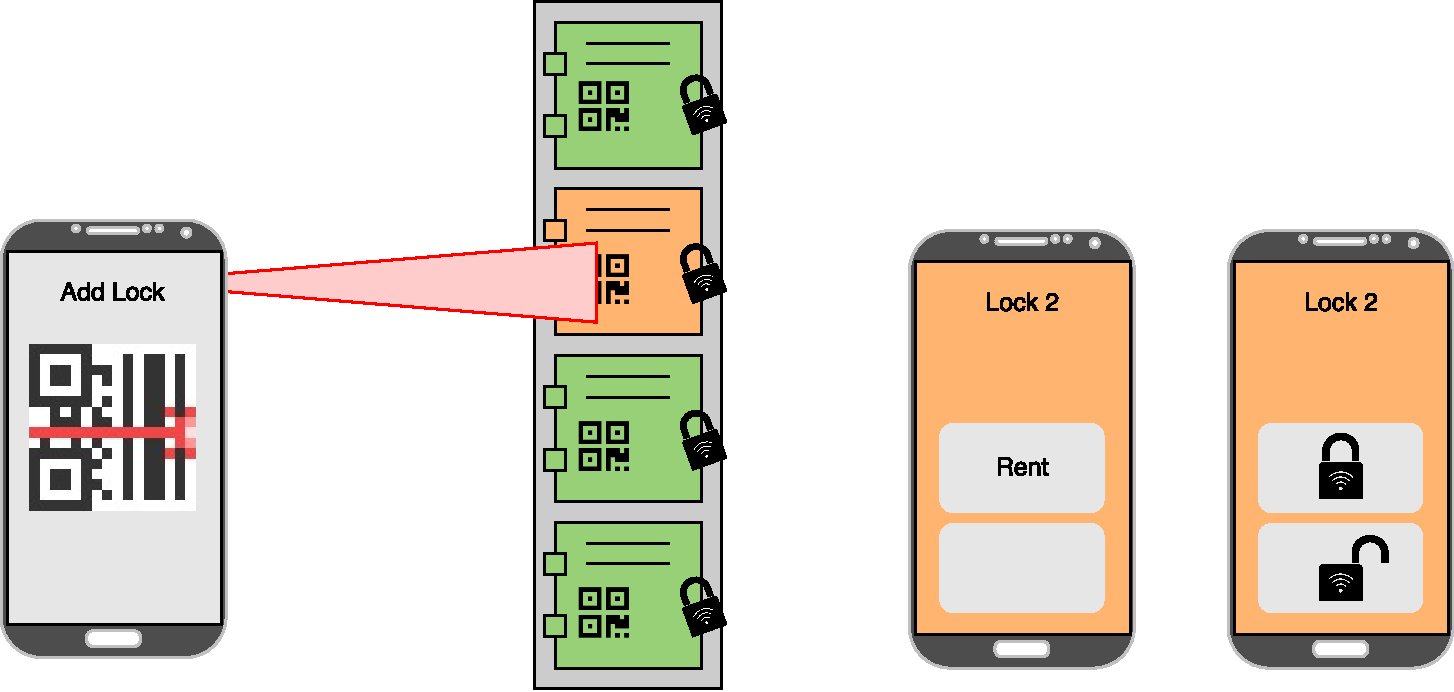
\includegraphics[width=.95\textwidth]{Mobile_Konzept}
\caption{Das Grobkonzept "Lokkit"}
\label{fig:Grobkonzept}
\end{figure}

In den nachfolgenden Abschnitten wird das Konzept weiter ausgeführt. Die System Spezifikation ist im Kapitel \ref{cha:Systemspezifikation} zu finden.

\subsection{Physischer Aufbau}
Jedes Schliessfach funktioniert autonom und besteht aus dem Schliessfach selbst, einem Raspberry Pi und einem Schloss. Das Raspberry Pi ist mit dem Schliessmechanismus verbunden und kann dieses auf Befehl hin Öffnen und Schliessen. Gleichzeitig wird eine Blockchain Node darauf ausgeführt und bildet im Verbund mit den anderen Raspberry Pis das private Netzwerk, das als Backend der Lösung fungiert.

Eines der Raspberry Pi's erstellt einen WLAN Hotspot und bietet DNS und DHCP Services für das Netzwerk an.

\paragraph{Autonomer Aufbau}
Grundsätzlich könnte auch einfach ein Rechner alle Schliessfächer steuern und Teil der privaten Blockchain sein. Diese Variante würde jedoch mehr einen zentralen Ansatz suggerieren und nicht den dezentralen Ansatz der Blockchain unterstreichen. Ausserdem besteht eine Blockchain aus mehreren Nodes, was den Einsatz von mehreren Raspberry Pis rechtfertigt. 
\paragraph{Raspberry Pi}
Die Raspberry Pis wurden vom Auftraggeber zur Verfügung gestellt. Es handelt sich um einen kompakten, vollständigen Computer, der das Ansteuern von Hardware (Schliessmechanismus) über den GPIO Pin ermöglicht. Ausserdem eignet es sich zum Erstellen eines eigenen Netzwerkes, das für die private Blockchain benötigt wird und verfügt über genügend Rechenpower um eine \emph{geth} Node (ohne Mining) laufen zu lassen.

\subsection{Interaktion mit dem Demonstrator}
\label{sec:Interaktion mit dem Demonstrator}

Ein Benutzer muss sich zuerst mit einer Node mit der Blockchain verbinden. Anschliessend kann er über die Webapp mit dem System interagieren.

\vspace{0.7em}\noindent
Folgende Interaktionen sind möglich.

\vspace{0.7em}\noindent
\textbf{Als Owner}
\begin{itemize}
    \item Ein neues Rentable erfassen
    \item Bestehende Rentables deaktivieren, aktivieren oder unbenutzbar machen
    \item Eigenschaften eines bestehenden Rentable ändern
    \item Rentable einem anderen Owner überschreiben
    \item Deposit von vergangenen Reservationen erhalten
\end{itemize}

\vspace{0.7em}\noindent
\textbf{Als potientieller Renter}
\begin{itemize}
    \item Informationen und Verfügbarkeit eines Rentables prüfen
    \item Ein Rentable reservieren (rent)
    \item Gutschriften abheben
\end{itemize}

\vspace{0.7em}\noindent
\textbf{Als aktueller Renter (current renter)}
\begin{itemize}
    \item Sperren und Entsperren des Rentables (Lock/Unlock)
    \item Zurückgeben des Rentables (unclaim, vgl. \ref{sys_para:claim_unclaim})
\end{itemize}

\subsection{Fallbeispiele}
\label{sec:Fallbeispiele}
Die folgenden beiden Fallbeispiele erläutern die Interaktion mit einem Schliessfach entlang der Zeitachse.

\subsubsection{Normal-Fall}
In Abb.~\ref{fig:Cases}\,(a) reserviert Benutzer A das Schliessfach von $t_{R1}$ bis $t_{R2}$ zum Zeitpunkt $t_0$. Das Deposit und die Mietkosten werden ihm somit abgezogen.
Zum Zeitpunt $t_{R1}$ wird Benutzer A zum \emph{Current Renter} und besitzt dadurch privilegierten Zugriff. Er kann jetzt das Schliessfach öffnen (Unlock) und schliessen (Lock). Nach einer gewissen Zeit noch vor Ablauf der Reservation, entschliesst sich Benutzer A das Schliessfach wieder abzugeben (Unclaim) (vgl. \ref{sys_subsubsec:Rentable}, speziell \ref{sys_para:claim_unclaim}), da er es nicht mehr benötigt. Die Reservation wird somit auf diesen Zeitpunkt gekürzt und Benutzer A erhählt sein Deposit und die Mietkosten für die ungenutzte Zeit teilweise zurück.

\begin{figure}
\centering\small
\setlength{\tabcolsep}{0mm}	% alle Spaltenränder auf 0mm
\begin{tabular}{c@{\hspace{12mm}}c} % mittlerer Abstand = 12mm
  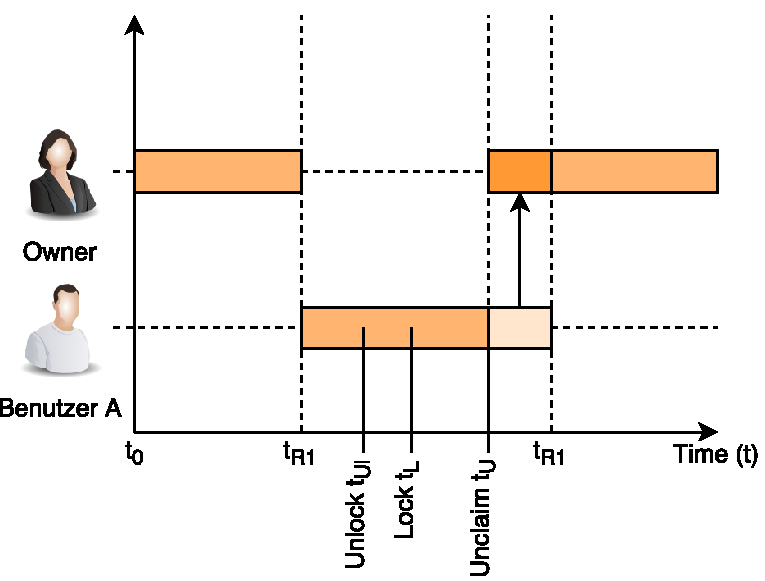
\includegraphics[width=.45\textwidth]{Case-Normal} &
  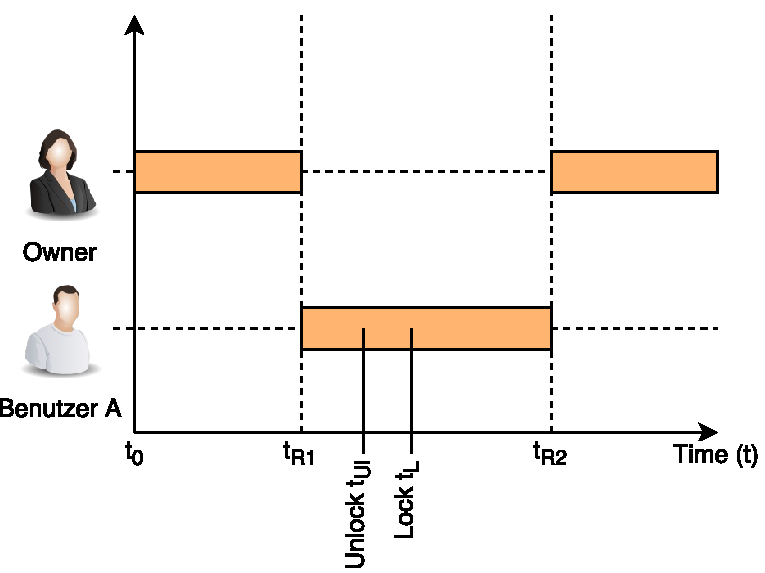
\includegraphics[width=.45\textwidth]{Case-No-Unclaim} \\
  (a) & (b) 
\end{tabular}
%
\caption{Verschiedene Fälle -- 
Normal-Fall (a), Keine-Rückgabe (b).}
\label{fig:Cases}
\end{figure}

%\begin{figure}
%\centering
%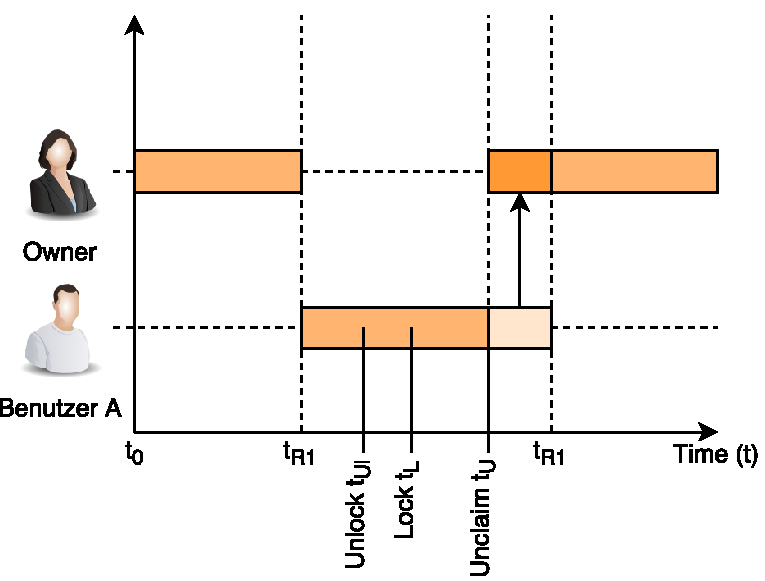
\includegraphics[width=.95\textwidth]{Case-Normal}
%\caption{Normal-Fall}
%\label{fig:Case-Normal}
%\end{figure}

\subsubsection{Reservationsende ohne Betätigung der Rückgabe}
Wie im Normal-Fall beschrieben, ist Benutzer A Current Renter des Schliessfaches. Anstatt das Schliessfach wieder zurückzugeben, lässt er die Reservationszeit auslaufen. Zum Zeitpunkt $t_{R2}$ werden ihm die Rechte entzogen und das Deposit wird nicht zurückerstattet. Es liegt also in Benutzer A seinem Interesse, alle eingeschlossenen Gegestände vor Ablauf der Reservation aus dem Schließfach zu nehmen und dieses zurückzugeben (Unclaim). Siehe Abb.~\ref{fig:Cases}\,(b) als Illustration.

\subsubsection{Fall von Schäden}
Benutzer A reserviert wie im Normalfall ein Schliessfach. Zum Zeitpunkt t1 will er das Schliessfach öffen (Unlock), dieses reagiert jedoch nicht. Er muss nun Kontakt mit dem Owner aufnehmen und die Sache klären. Auf jeden Fall sollte er nun das Schliessfach zurückgeben (Unclaim), um seine Kosten gering zu halten, im Falle, dass der Owner nicht kontaktierbar ist oder dieser kein Interesse zeigt.

Ein mögliches Konzept, wie solche Probleme vermindert werden könnten, wäre z.B. das Einführen eines Review Systems, wo Benutzer die Owner beurteilen könnten. Owner mit einer guten Bewertung (Score) wären dann vertrauenswürdiger. Im Rahmen dieser Arbeit wurde dies aber nicht mehr weiter ausgeführt. 

\subsection{Sicherheit}
Im Design und bei der Umsetzung dieses Systems wurde angenommen, dass die Implementation des gesamten Ethereum Protokolls und der Web3 Funktionen kryptographisch sicher ist. Die Validität eines Smart Contracts sollte nicht infrage gestellt werden, sofern die Blockchain in einem validen Zustand ist.\cite{github.com/ethereum/web3js, go-ethereum}

Der einzige selbst entwickelte sicherheitskritische Aspekt ist bei der Übermittlung der Nachrichten mittels Whisper v5 (vgl. \ref{para:Whisper}). Entsprechend findet sich im Kapitel \ref{subsubsec:Sicherheitsaspekte} eine Abhandlung der gemachten Überlegungen und getroffene Massnahmen zur Sicherstellung der validen Herkunft der Nachrichten.